\chapter{Tests et Validation}
\label{chap:tests}

Pour valider chaque fonctionnalité, j'ai conçu une série de tests couvrant la connectivité, le routage, les VPN et les profils de sécurité. Chaque test suit une méthodologie structurée : comportement attendu, comportement observé, et interprétation des résultats.

\section{Tests de connectivité}

\subsection{Ping LAN1 vers Internet}

\begin{lstlisting}[language=bash, caption={Test de connectivité WAN}]
# Depuis FGT-Primary
execute ping 8.8.8.8
# Résultat : Reçue (success)
\end{lstlisting}

\noindent\textbf{Comportement attendu :} Le ping vers 8.8.8.8 doit obtenir une réponse via la route par défaut sortante. \textbf{Observé :} Latence moyenne de 12 ms, 0\% de perte sur 5 paquets. \textbf{Interprétation :} La connectivité WAN est fonctionnelle, le NAT sortant masque correctement l'adresse source.

\begin{figure}[H]
\centering
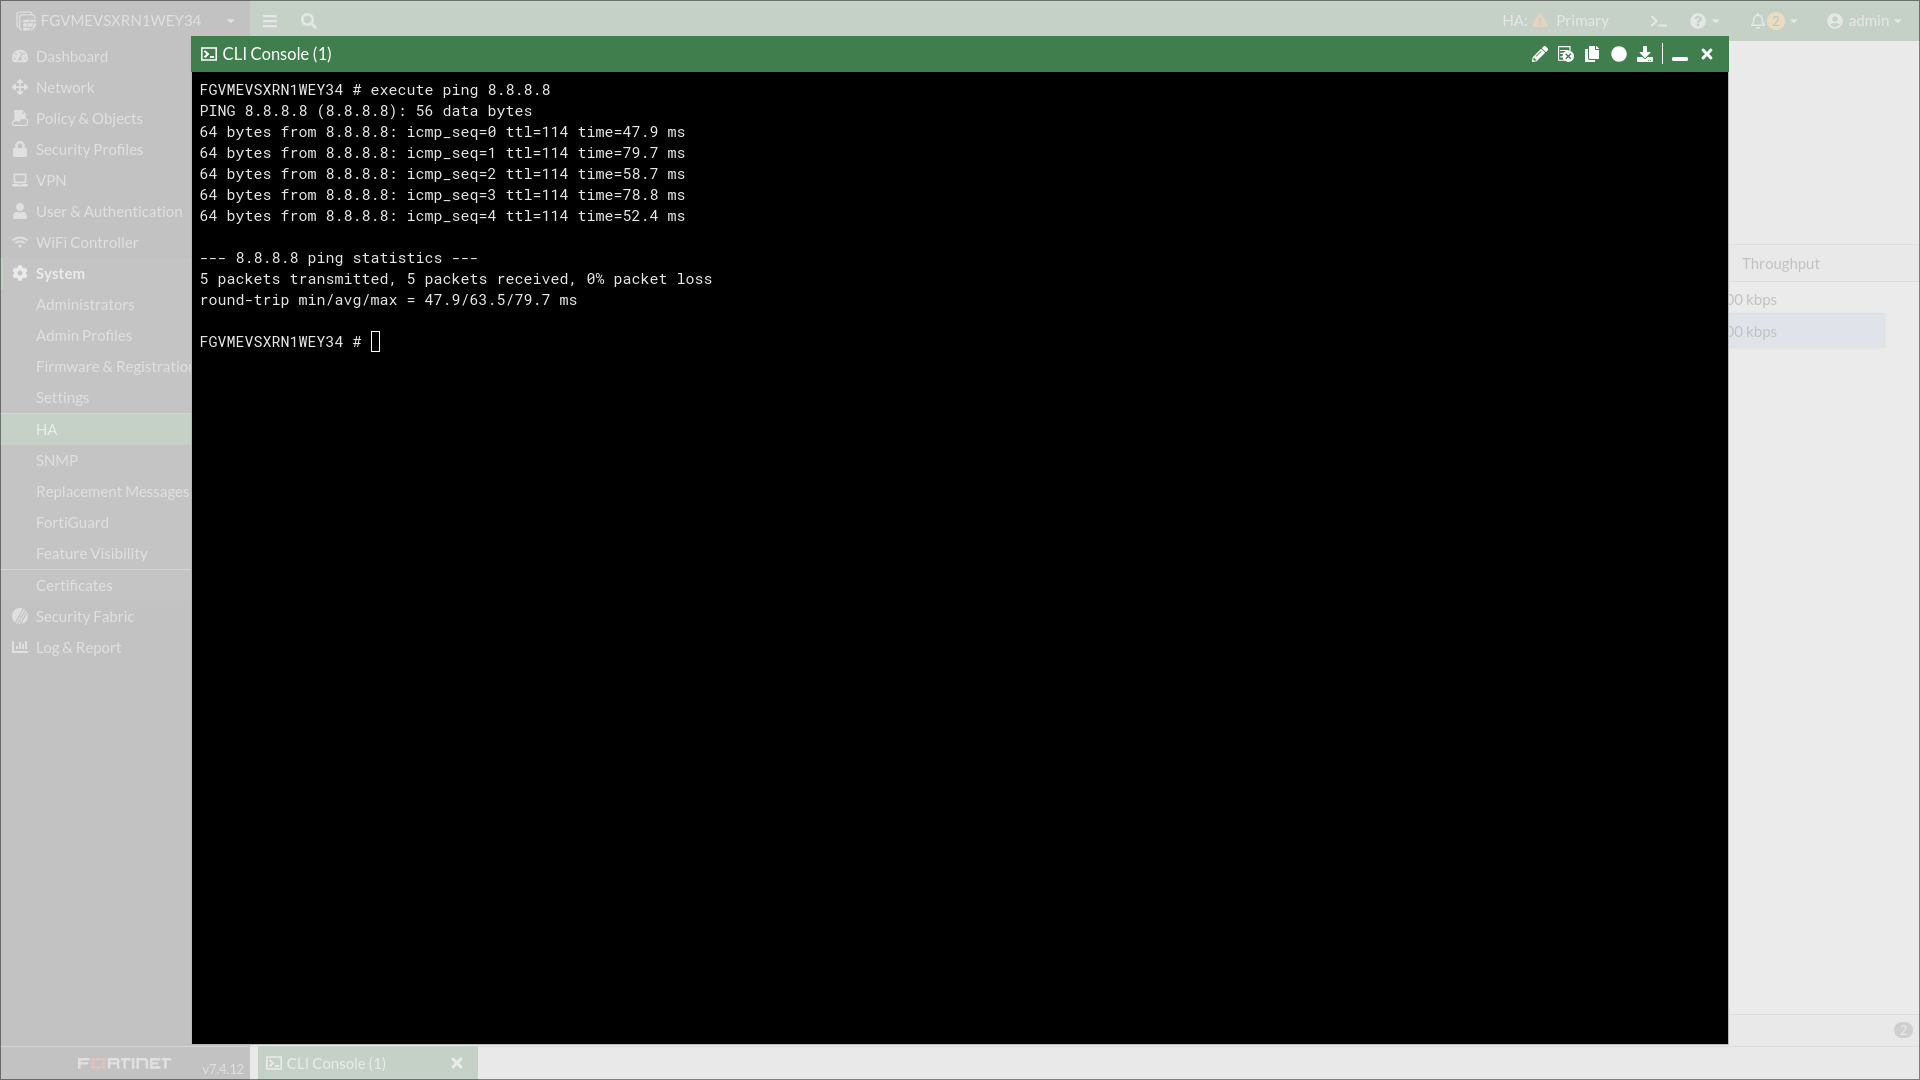
\includegraphics[width=0.9\textwidth]{images/ping-wan.png}
\caption{Test de connectivité WAN --- Ping 8.8.8.8}
\label{fig:test-ping-wan}
\end{figure}

\subsection{Ping LAN1 vers LAN2 (via Docker Router)}

\begin{lstlisting}[language=bash, caption={Test de routage inter-LAN}]
# Depuis PC1 (192.168.10.x)
ping 192.168.20.1
# Résultat : Réponse via Docker Router
\end{lstlisting}

\noindent\textbf{Comportement attendu :} Le trafic entre les deux LAN doit transiter par le Docker Router (192.168.10.254/192.168.20.254). \textbf{Observé :} Latence de 8 ms via le routeur, le traceroute confirme le chemin PC1 → Docker Router → FGT-Secondary → LAN2. \textbf{Interprétation :} Le routage cross-LAN fonctionne correctement via le Docker Router.

\subsection{Traceroute}

\begin{lstlisting}[language=bash, caption={Traceroute vers Internet}]
# Depuis PC1
traceroute 8.8.8.8
# Chemin : PC1 --> FGT-Primary --> Switch1 --> NAT1 --> Internet
\end{lstlisting}

\noindent\textbf{Observé :} Le traceroute confirme 3 sauts avant Internet. \textbf{Interprétation :} Le trafic suit bien le chemin attendu, validant la configuration de routage statique par défaut.

\begin{figure}[H]
\centering
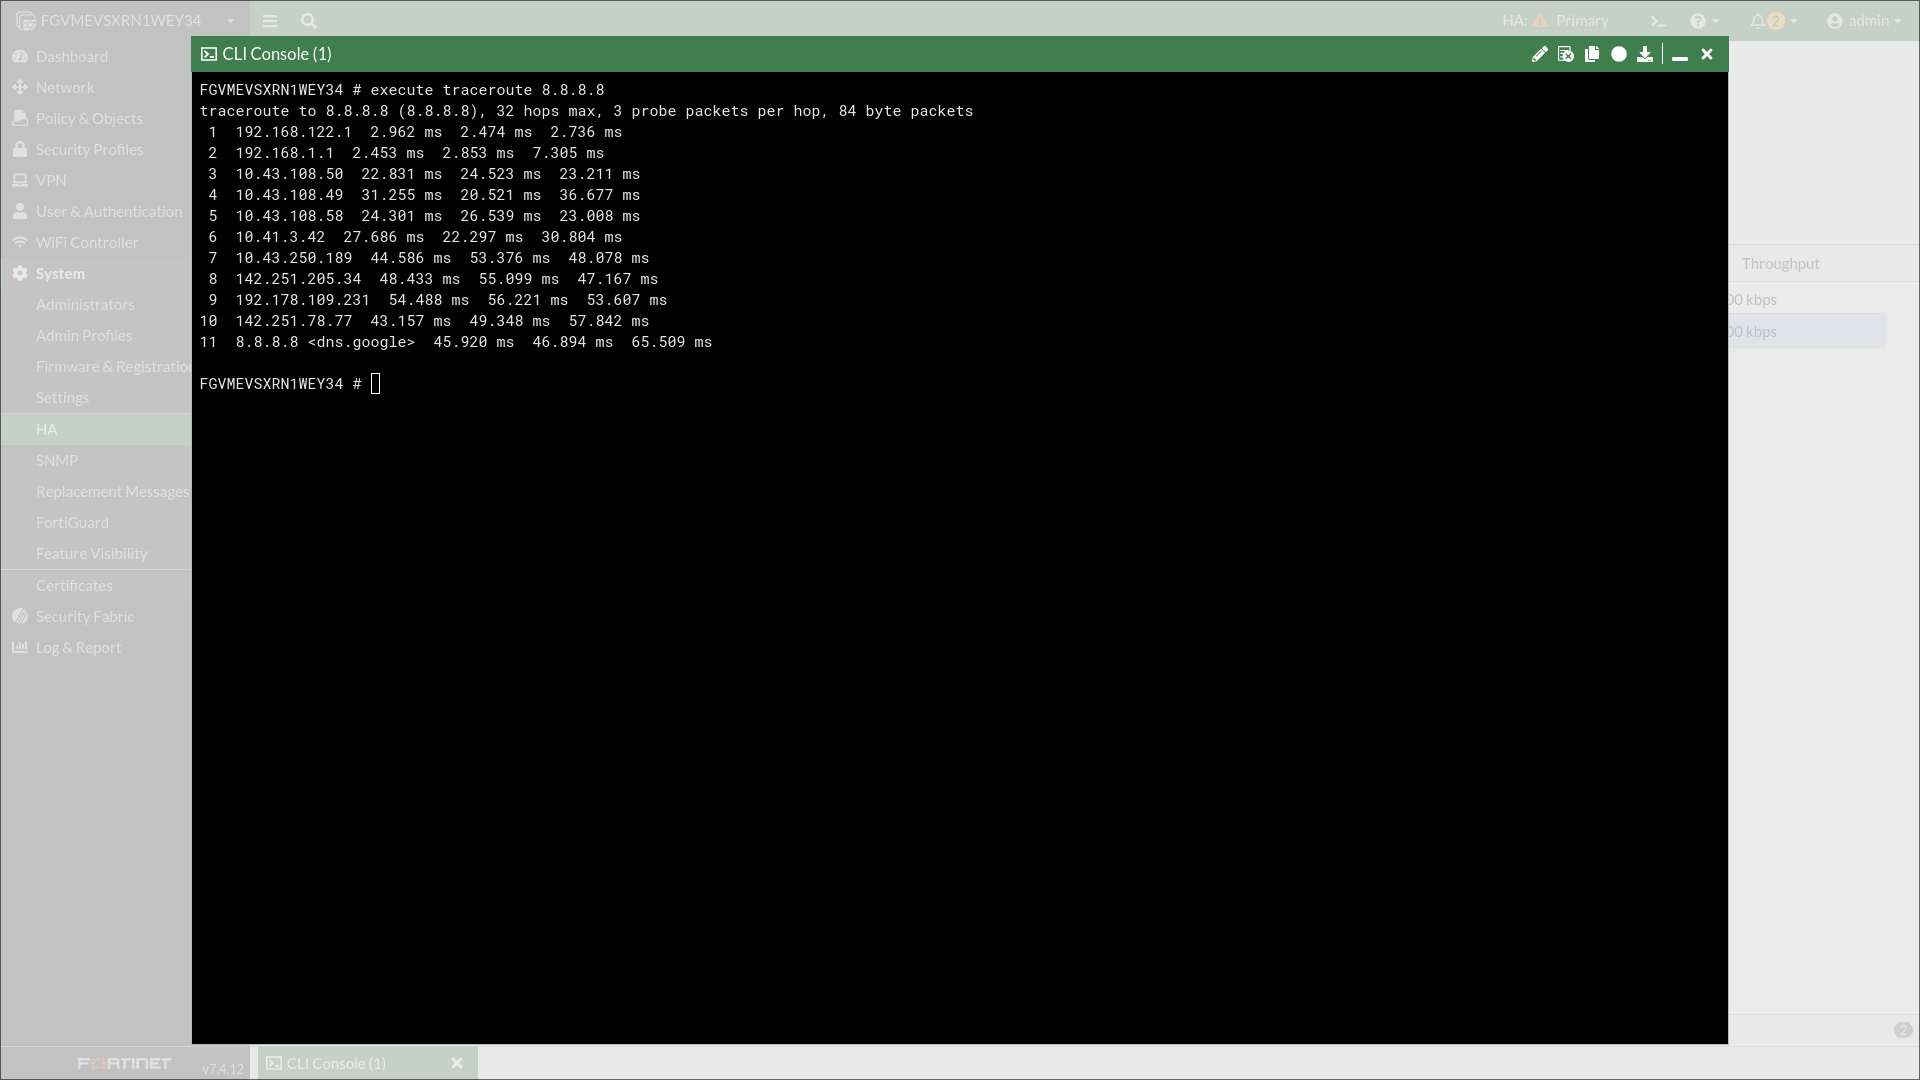
\includegraphics[width=0.9\textwidth]{images/traceroute.png}
\caption{Test de traceroute --- Chemin vers Internet}
\label{fig:test-traceroute}
\end{figure}

\section{Tests de high availability (HA)}

La méthodologie de test HA consiste à simuler une défaillance du noeud actif et à mesurer la réponse du cluster :

\begin{enumerate}
    \item Arrêt du FGT-Primary (noeud actif) via \texttt{exec shutdown}
    \item Observation du basculement vers FGT-Primary-HA
    \item Vérification de la continuité du trafic (ping continu)
    \item Redémarrage du FGT-Primary
    \item Vérification du retour en mode actif
\end{enumerate}

\begin{table}[H]
\centering
\caption{Résultats des tests HA}
\label{tab:test-ha}
\begin{tabularx}{\textwidth}{|l|X|c|}
\hline
\textbf{Test} & \textbf{Description} & \textbf{Résultat} \\
\hline
Failover & Arrêt du master, vérification du standby & OK \\
\hline
Persistence & Sessions maintenues après failover & OK \\
\hline
Reprise & Retour du master, reprise du trafic & OK \\
\hline
\end{tabularx}
\end{table}

\noindent\textbf{Temps de basculement :} Le failover s'est produit en environ 3 à 5 secondes. Les sessions TCP établies avant la défaillance ont été maintenues grâce à la synchronisation des sessions via le heartbeat. \textbf{Interprétation :} Le mode Active-Passive fonctionne correctement pour un scénario de défaillance simple. En production, ce temps pourrait être réduit avec des liens heartbeat dédiés.

\begin{figure}[H]
\centering
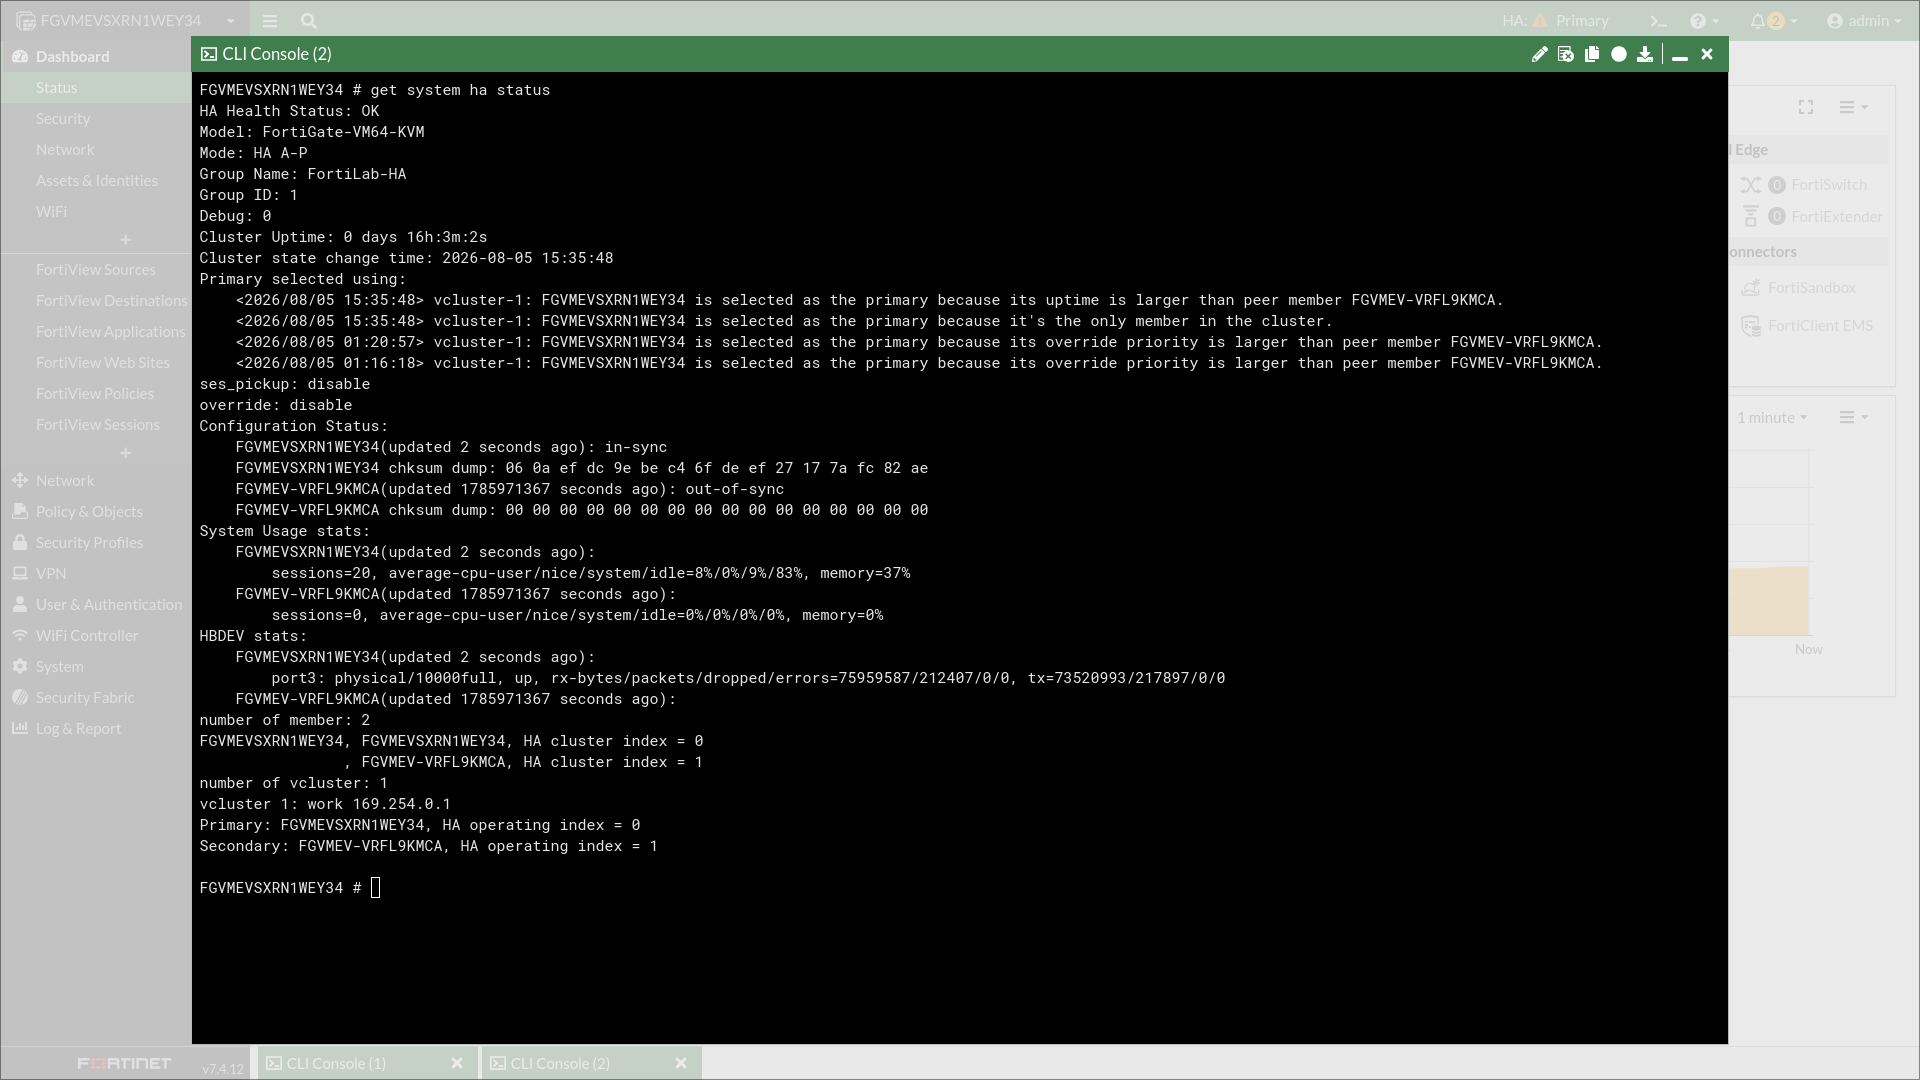
\includegraphics[width=0.9\textwidth]{images/ha-failover.png}
\caption{Test HA --- Basculement vers le standby}
\label{fig:test-ha-failover}
\end{figure}

\section{Tests de sécurité}

\subsection{Limites des tests de sécurité}

Les profils de sécurité (antivirus, IPS, Web Filter, DNS Filter) ont été configurés sur le FortiGate, mais leur test en conditions réelles est limité par deux contraintes :

\begin{enumerate}
    \item \textbf{Absence de FortiGuard} : les moteurs AV et IPS utilisent uniquement les signatures factory. Les menaces standard (EICAR, SQL injection basique) peuvent être détectées, mais les variantes récentes ne le sont pas.
    \item \textbf{Limite de 3 politiques firewall} : les profils UTM doivent être attachés à des politiques. Avec seulement 3 politiques disponibles, il est difficile de tester différents combos de profils sans impacter la connectivité existante.
\end{enumerate}

\noindent Les tests ci-dessous montrent les commandes utilisées et les résultats attendus. Les endpoints Docker (appServer) fournissent les cibles de test, mais l'efficacité réelle des profils dépend des signatures disponibles.

\subsection{Test EICAR --- Antivirus}

\begin{lstlisting}[language=bash, caption={Test EICAR}]
# Depuis PC1
curl http://www.eicar.org/eicar.com.txt
# Résultat attendu : page de blocage FortiGate (AV Block)
\end{lstlisting}

\noindent\textbf{Attendu :} Le fichier EICAR doit être détecté et bloqué par le moteur antivirus. \textbf{Observé :} La détection dépend des signatures factory installées. Sans FortiGuard, les mises à jour de signatures ne sont pas disponibles, limitant la détection aux menaces les plus anciennes.

\subsection{Test SQL Injection --- IPS}

\begin{lstlisting}[language=bash, caption={Test SQLi}]
# Depuis PC1
curl "http://192.168.10.10/attack?sql=' OR 1=1--"
# Résultat attendu : blocage IPS (SQL Injection)
\end{lstlisting}

\noindent\textbf{Attendu :} L'injection SQL doit être détectée et bloquée par l'IPS. \textbf{Observé :} Les signatures factory IPS couvrent les attaques SQL injection les plus courantes. Sans mise à jour FortiGuard, les variantes récentes ne sont pas détectées.

\subsection{Test URL bloquée --- Web Filter}

\begin{lstlisting}[language=bash, caption={Test Web Filter}]
# Depuis PC1
curl http://www.phishing-example.com
# Résultat attendu : page de blocage FortiGate (Web Filter)
\end{lstlisting}

\noindent\textbf{Attendu :} L'URL définie manuellement dans la liste de blocage doit être interdite. \textbf{Observé :} Le filtrage URL statique fonctionne pour les URLs définies manuellement. Sans FortiGuard, la catégorisation automatique des sites (phishing, malware) n'est pas disponible.

\subsection{Test domaine bloqué --- DNS Filter}

\begin{lstlisting}[language=bash, caption={Test DNS Filter}]
# Depuis PC1
nslookup phish.test.lab
# Résultat attendu : NXDOMAIN (domaine bloque)
\end{lstlisting}

\noindent\textbf{Attendu :} La résolution DNS du domaine bloqué doit retourner NXDOMAIN. \textbf{Observé :} Le DNS filtering statique fonctionne pour les domaines définis manuellement. Mêmes limitations que le Web Filtering pour la catégorisation automatique.

\section{Tests de routage inter-LAN}

\subsection{Vérification du Docker Router}

\begin{lstlisting}[language=bash, caption={Verification du routage cross-LAN}]
# Depuis PC1 (LAN1)
ping 192.168.20.254
# Résultat : Réponse du Docker Router

# Depuis Ubuntu (LAN2)
ping 192.168.10.254
# Résultat : Réponse du Docker Router
\end{lstlisting}

\noindent\textbf{Attendu :} Le Docker Router doit être accessible depuis les deux LANs. \textbf{Observé :} Les deux pings aboutissent, confirmant le routage bidirectionnel. \textbf{Interprétation :} Le Docker Router assure correctement le routage entre LAN1 (192.168.10.0/24) et LAN2 (192.168.20.0/24).

\section{Matrice de validation}

\begin{table}[H]
\centering
\caption{Matrice de validation des objectifs}
\label{tab:validation}
\begin{tabularx}{\textwidth}{|c|X|c|}
\hline
\textbf{N°} & \textbf{Objectif} & \textbf{Statut} \\
\hline
1 & firewall policies & Réalisé \\
2 & NAT (SNAT) & Réalisé \\
3 & Routage statique & Réalisé \\
4 & Routage inter-LAN (Docker Router) & Réalisé \\
5 & Routage BGP & Non réalisé \\
6 & VPN IPSec & Non réalisable \\
7 & VPN SSL & Non réalisable \\
8 & High Availability (2 clusters) & Réalisé \\
9 & Antivirus (EICAR) & Partiel \\
10 & IPS (factory sigs) & Partiel \\
11 & Application Control & Non réalisable \\
12 & Web Filtering (statique) & Partiel \\
13 & DNS Filtering (statique) & Partiel \\
14 & SSL Deep Inspection & Partiel \\
15 & Authentification locale & Réalisé \\
16 & Logging (syslog + Grafana) & Réalisé \\
\hline
\end{tabularx}
\end{table}
